\documentclass[11pt,letterpaper]{article}
\usepackage[margin=1in]{geometry}
\usepackage[utf8]{inputenc}
\usepackage[T1]{fontenc}
\usepackage{amsmath,amssymb}
\usepackage{graphicx}
\usepackage{booktabs}
\usepackage{natbib}
\usepackage[colorlinks=true,linkcolor=black,citecolor=black,urlcolor=black]{hyperref}
\usepackage{url}
\usepackage{caption}
\makeatletter
\g@addto@macro{\UrlBreaks}{\UrlOrds}
\makeatother
\usepackage{multirow}
\usepackage{array}
\usepackage{xcolor}
\setlength{\emergencystretch}{2em}

\title{Early co-occurrence network openness is associated with cross-disciplinary concept breadth: evidence from 12,499 scientific concepts}

\author{AI Inventor}

\date{}

\begin{document}

\maketitle

\begin{abstract}
We ask which early structural signals in a concept's topic co-occurrence network anticipate later cross-field breadth. Using the OpenAlex bulk snapshot, we identify 12,499 concepts across 26 scientific fields and screen 53 early network indicators from six families against a popularity baseline on held-out field groups. Seven indicators survive held-out validation, three of them ego-network measures. From the ego-network family we build a six-component openness index (OPEN) that measures a concept's early tendency to acquire novel, community-spanning co-occurrence partners. Pooled across six non-selection bodies, the partial Spearman correlation of the home-field OPEN index with rarefied breadth is $+0.069$ $[+0.038, +0.100]$ ($I^2 = 0$, all bodies positive; a single descriptive estimate). The association behaves like a static topical-dispersion property: a within-concept permutation null absorbs year-to-year churn, but the temporal-excess measure is too unreliable to adjudicate, so temporal turnover is untested rather than refuted. Separately, a conditional logit on an independent frame of field-entry events shows that concepts spread next to fields related to the ones currently retaining them ($d_0 = 0.322$ $[0.291, 0.355]$), but the pre-registered verdict is partial: the volume-matched contrast is null and the coefficient reverses under an alternative proximity measure. In an accounting decomposition, early contact diversity accounts for most of the breadth gap; no discrete trajectory typology is stable.
\end{abstract}

\noindent\textbf{Keywords:} co-occurrence networks, cross-disciplinary diffusion, knowledge spread, principle of relatedness, scientific concepts, temporal networks, topic emergence


\section{Background}
\label{sec:background}

Some scientific concepts remain confined to their home discipline for decades, while others cross field boundaries within a few years. Optogenetics, born in neuroscience, entered genetics, psychiatry and bioengineering; deep learning, rooted in computer science, now appears in medicine, materials science and linguistics. Understanding what distinguishes broadly spreading concepts from locally absorbed ones matters for science policy, research evaluation and the design of interdisciplinary programmes \citep{Fortunato2018,Hofstra2019}. If early structural signals predict later cross-field integration, funders and institutions could identify concepts with high diffusion potential before that diffusion is observable in publication counts alone.

The problem is hard because simple popularity metrics (publication volume, growth rate, share of papers outside the home field) already explain much of the variance in later breadth \citep{Rotolo2015}. Any network indicator must add information \emph{beyond} these baselines. Network science offers a rich toolkit for studying how information, behaviour and innovations spread through structured populations \citep{Milli2018}. Spreading outcomes depend on both the topology of the network and the position of the spreading entity within it, including in multilayer settings \citep{Domenico2016}, and knowledge flows through citation networks follow structured pathways \citep{Renoust2017}. Community structure shapes diffusion outcomes: bridge nodes and boundary-spanning ties accelerate spread across groups \citep{Cherifi2019,Burt2004}, while community cohesion can either facilitate or retard it depending on the contagion mechanism \citep{Centola2010,Ugander2012}.

Prior work has proposed several candidate signals for concept diffusion. \citet{Cheng2023} followed about 60{,}000 new ideas across 38 million papers and found that ideas become ``core'' when they reach networks of unrelated authors and fit existing research traditions. Their ideational consistency measure predicted next-year volume. \citet{Weng2013} showed that the community structure of a meme's early adopters predicts its virality, about seven times as precisely as random guessing. \citet{Salatino2017} showed that collaboration among existing topics intensifies before a new topic emerges, and \citet{Chavalarias2013} used phylomemetic methods to track the branching and merging of scientific fields. \citet{Gao2018} tracked community evolution in patent co-occurrence networks, revealing how technological change reshapes network structure. \citet{Sattar2023} developed approaches for detecting the temporal evolution of communities, and \citet{Callon1991} introduced co-word analysis as a tool for mapping research structure. These studies typically operate on curated concept sets without held-out validation, mix concept-level and field-level units of analysis, or do not control for simple volume-based predictors. No prior study has screened a broad set of temporal knowledge-network indicators against a shared baseline on held-out field groups for the specific outcome of size-adjusted cross-disciplinary breadth.

A second open question concerns the routes by which concepts move between fields. The principle of relatedness, established for regional economic diversification \citep{Hidalgo2007,Boschma2015}, predicts that actors diversify into activities related to their existing portfolio. For scientific fields adopting new concepts, this principle has been tested for entry but not for the role of currently \emph{retaining} fields---those that have adopted a concept and kept publishing on it. Whether concepts spread next to fields related to the ones currently retaining them, beyond relatedness to the home field alone, is untested.

This paper addresses both questions with a large-scale empirical study (Figure~\ref{fig:overview}). We identify 12{,}499 concepts from the OpenAlex bulk snapshot, compute 53 early network indicators across six families, and test them on held-out field groups and a confirmatory onset cohort. We also build a conditional logit model of field entry that tests whether retained-field relatedness predicts the next field a concept enters. We report the following contributions:

\begin{enumerate}
    \item We screen 53 early co-occurrence network indicators against a five-feature popularity baseline and confirm seven on held-out field groups for predicting rarefied cross-field breadth. Two of the seven carry negative signs: early retention ratio and ego-network density.
    \item We introduce the OPEN index, a six-component composite of early co-occurrence openness, and test it on a 2015--2017 cohort never used in selection. Pooled across six non-selection bodies, OPEN$_{\text{home}}$ gives partial Spearman +0.069 [+0.038, +0.100], $I^2 = 0$, all bodies positive (a descriptive estimate).
    \item We test whether concepts spread next to fields related to the ones currently retaining them. On an independent frame (11,841 concepts, 6,978 entry events in 6,076 informative strata), the retained-frontier coefficient is $d_0 = +0.322$ $[+0.291, +0.355]$. The pre-registered verdict is partial: the volume-matched contrast is null, the coefficient reverses under minimum-conditional-probability proximity, and the held-out dose response is not monotone. Persistence and volume remain confounded.
    \item We show that early neighbourhood consolidation, measured by \citeauthor{Cheng2023}'s (\citeyear{Cheng2023}) ideational consistency, predicts volume growth but \emph{narrower} cross-field reach, a reversal that holds in all five field groups of the selection frame but is not confirmed on the vocabulary-free frame.
    \item We decompose breadth into exploration and retention channels and show, as an accounting identity, that early exploration accounts for about three-quarters of the breadth gap (73\% in the unstratified decomposition, almost all of it early contact diversity). No discrete trajectory typology passes the naming rule; diffusion paths form a continuum along a breadth axis.
\end{enumerate}

\begin{figure}[!htbp]
  \centering
  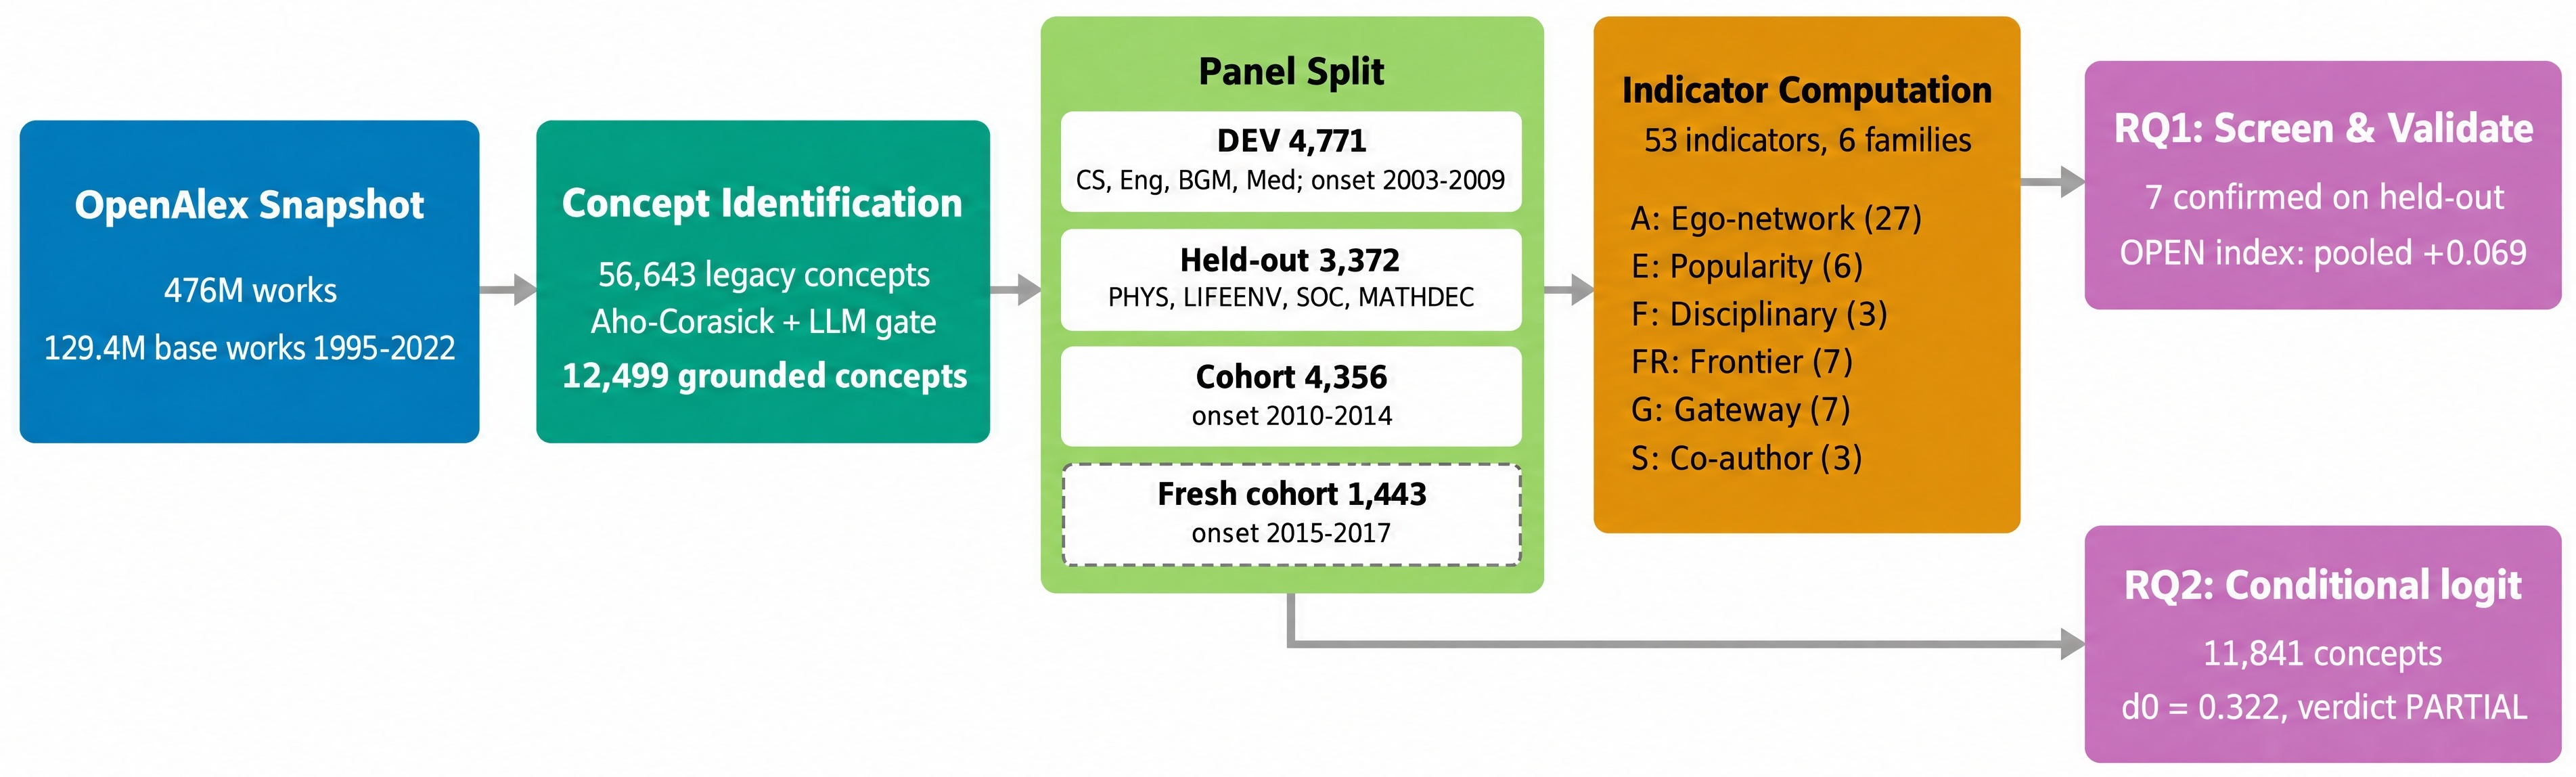
\includegraphics[width=\linewidth,height=0.85\textheight,keepaspectratio]{figures/fig_overview_v0.jpg}
  \caption{Overview of the study design, read left to right. The OpenAlex snapshot (blue; 476M works, 129.4M base works 1995--2022) is title-matched against 56,643 legacy concepts, and Aho--Corasick matching plus an LLM precision gate (teal) keeps 12,499 grounded concepts. The panel split (green) assigns these to a development set (DEV 4,771; CS, Eng, BGM, Med homes, onset 2003--2009), four held-out domain groups (3,372; PHYS, LIFEENV, SOC, MATHDEC) and a 2010--2014 onset cohort (4,356). A fresh 2015--2017 cohort (1,443; dashed box) comes from a separate scan. For each concept, 53 early indicators in six families (orange; A ego-network 27, E popularity 6, F disciplinary 3, FR frontier 7, G gateway 7, S co-author 3) are computed in the $t_0$ to $t_0{+}2$ window. They are screened on DEV and validated on held-out groups (RQ1, top right): 7 frozen indicators are confirmed on held-out, and the pooled partial Spearman of the OPEN index is $+0.069$. Separately (lower arrow, bypassing the indicators), a conditional-logit entry model is fitted on an independent concept frame of 11,841 concepts (RQ2, bottom right). It gives $d_0 = 0.322$ for retained-frontier relatedness, and the pre-registered verdict is PARTIAL because persistence is confounded with volume.}
  \label{fig:overview}
\end{figure}


\section{Methods}
\label{sec:methods}

\subsection{Concept identification and panel construction}

We use the OpenAlex bulk snapshot (2026-09-23; 476{,}196{,}327 works; 129.4 million base works 1995--2022). Concepts are identified by Aho--Corasick title matching of 56{,}643 legacy OpenAlex concepts (levels 2--5) plus Wikidata aliases, with stemmed verification. A per-concept LLM precision gate drops concepts with precision below 0.80.

A concept's \emph{onset year} $t_0$ is the first year it reaches 20 grounded publications. \emph{Home field(s)} are the field(s) holding at least 40\% of the first 30 grounded papers. The specification was frozen on DEV data (hash-sealed before held-out scoring) and unsealed once. The panel comprises 12{,}499 concepts and 27{,}393 concept-by-field adoption episodes (Table~\ref{tab:panel}).

\begin{table}[!htbp]
\centering
\caption{Panel composition. DEV concepts have home fields in Computer Science, Engineering, Biochemistry/Genetics/Medicine. Held-out groups cover the remaining field families.}
\label{tab:panel}
\small
\begin{tabular}{lrr}
\toprule
Split & Concepts & Episodes \\
\midrule
DEV (CS/Eng/BGM/Med, onset 2003--2009) & 4{,}771 & 9{,}079 \\
Cohort (onset 2010--2014, all fields) & 4{,}356 & 9{,}799 \\
Held-out Physical Sciences & 742 & 1{,}662 \\
Held-out Life \& Environment & 1{,}113 & 3{,}099 \\
Held-out Social Sciences & 1{,}352 & 3{,}320 \\
Held-out Math \& Decision Sci. & 165 & 434 \\
\midrule
\textbf{Total} & \textbf{12{,}499} & \textbf{27{,}393} \\
\bottomrule
\end{tabular}
\end{table}

\subsection{Outcome: rarefied field breadth}

The primary outcome is \emph{rarefied field breadth} $O_{2r}$ ($m = 50$): the expected number of distinct venue fields among a fixed-size random draw of $m$ papers from a concept's publications in years $t_0 + 6$ to $t_0 + 8$, computed by exact hypergeometric rarefaction. Rarefaction separates size-adjusted breadth from sheer volume. Secondary outcomes include sustained uptake ($O_{1c}$), transience ($O_3$), and field- and year-normalised citation growth ($O_4$).

\subsection{Baseline and indicator families}
\label{sec:indicators}

We define a \emph{five-feature baseline} (B5) consisting of log early volume, publication growth, non-home share, Shannon entropy and field reach, all computed over $t_0$ to $t_0 + 2$. The 53 candidate indicators span six families:

\begin{enumerate}
    \item \textbf{Co-occurrence ego-network (A, 27 indicators):} degree, density, persistence, novelty, community counts, participation, brokerage from the concept's ego network on the co-occurrence backbone.
    \item \textbf{Popularity and volume (E, 6 indicators):} share, growth, acceleration, burst, author growth, author count.
    \item \textbf{Disciplinary spread (F, 3 indicators):} log off-home volume, Rao--Stirling diversity of venue fields, fields gained per year.
    \item \textbf{Retained frontier (FR, 7 indicators):} contact reach, retained reach, retention ratio, frontier potential, and RCA-based, volume-weighted and Hidalgo field densities at $t_0{+}2$ (the last three use cumulative field history from 1995).
    \item \textbf{Gateway and landing (G, 7 indicators):} gateway-weighted early landing (eigenvector, betweenness, degree and $\phi_{\min}$ variants), home relatedness of landing fields, and Rao--Stirling diversity with $1-\phi_{\min}$ distances.
    \item \textbf{Co-author structure (S, 3 indicators):} connected components of the early co-author graph, their size-normalised count, and the share of isolated authors.
\end{enumerate}

\subsection{The OPEN index}

The OPEN index is the mean of six signed $z$-scored ego-network components from the early window ($t_0$ to $t_0 + 2$):

\begin{enumerate}
    \item New edge rate (positive sign): the fraction of a concept's co-occurrence neighbours that are new.
    \item Number of Leiden communities reached ($n_{\text{comm}}$, positive): how many distinct topic communities a concept's neighbours span.
    \item Participation coefficient (positive): the share of a concept's ties that cross community boundaries.
    \item Neighbourhood novelty residual (NOV$_{\text{res}}$, positive): the novelty of a concept's co-occurrence partners after residualising on degree.
    \item Ego density (negative sign): the density of the concept's local co-occurrence subgraph.
    \item Edge persistence (negative sign): the fraction of the concept's neighbours retained across windows.
\end{enumerate}

The $z$-score constants are frozen on the 12{,}499-concept frame (selection data) before any confirmation body is scored. We test three builds: OPEN$_{\text{home}}$ (home-field co-occurrence graph only), OPEN$_{\text{all}}$ (corpus-wide graph), and OPEN$_{\text{sizematch}}$ (corpus-wide papers subsampled to home counts).

\subsection{Statistical framework}

Indicator screening uses \emph{partial Spearman priority} (PSP): the Pearson correlation of rank-transformed indicator and outcome residuals, both residualised on the baseline covariates and control rungs. Inference uses 2{,}000 concept-level bootstrap resamples with refit. Pooling across field groups uses the DerSimonian--Laird random-effects estimator \citep{Dersimonian1986} with $I^2$ heterogeneity reporting \citep{Higgins2002}. Multiple comparisons use Holm correction across the pre-declared family.

We also define NOVCHURN as the mean of $z$(NOV$_{\text{res}}$) and $-z$(edge persistence), a two-component novelty/churn measure used in mechanism analyses.

\subsection{Field-entry model}

For the field-entry analysis, we use a conditional logit (Breslow partial likelihood) on concept-year risk sets, stratified by concept-year, with standardised covariates: relatedness to home, log field size, density over entered fields, gateway centrality (baseline R0); RCA-based density (R1); volume-weighted density (R2); and retained-field relatedness $d_0$ (R3). A field is ``retaining'' a concept in year $t$ when it is off-home, had entered by $t-2$ (at least two cumulative grounded papers) and has published at least two grounded papers on the concept over $t-2$ to $t$. Relatedness is measured by positive pointwise mutual information (PMI) on the field-level backbone. The specification is frozen on DEV and scored once on the independent held-out frame.


\section{Results}
\label{sec:results}

The headline finding is the openness--breadth association: pooled across six non-selection bodies, OPEN$_{\text{home}}$ gives partial Spearman $+0.069$ $[+0.038, +0.100]$, $I^2 = 0$, all six positive (a descriptive estimate). We present the indicator screen first because it defines the OPEN index.

\subsection{Which early network signals predict cross-field breadth?}

\subsubsection{Experimental setup}

The top 10 indicators selected on DEV by partial Spearman priority for rarefied breadth ($O_{2r}$, $m = 50$) were tested once on four held-out field groups and two cohort splits\footnote{Code: \url{https://github.com/ai-inventor-papers/ai-invention-8795ea-concepts-spread-once-adopters-make-them/tree/fork/run_-IpcIodNqp66/round-3/experiment-8}}. Confirmation requires Holm-corrected $p < 0.05$ and a 95\% CI excluding zero on the DerSimonian--Laird pooled estimate. The held-out outcomes had been previously used by two earlier experiments, so the indicator-screen results are robustness checks within the same frame rather than fully independent confirmations. The fresh 2015--2017 cohort is the only body never used in any prior step.

\subsubsection{Comparison to related work}

Prior network-based diffusion studies have examined spreading processes on multilayer networks \citep{Domenico2016}, knowledge flow through citation networks \citep{Renoust2017}, community-driven diffusion mechanisms \citep{Cherifi2019,Milli2018}, and temporal community evolution \citep{Sattar2023,Gao2018}. These studies model diffusion at the network level but do not screen concept-level co-occurrence indicators against a held-out validation framework for the specific outcome of size-adjusted breadth. \citet{Weng2013} showed that early community structure predicts online virality (about seven times random precision); our study extends this to scientific concepts, where the baseline is much stronger (B5 Spearman 0.65--0.86). \citet{Cheng2023} found that reaching unrelated author networks predicts whether ideas become ``core,'' but did not control for a shared baseline or use held-out field groups. \citet{Fitzgerald2021} asked whether academic collaboration is becoming more localised, motivating the question of which early signals distinguish concepts that overcome this localisation.

\subsubsection{Results}

Seven of the 53 screened indicators survive held-out validation with Holm correction (Table~\ref{tab:screen}). These span two families: retained frontier (end-of-window field density, volume-weighted field density, contact reach, retention ratio) and co-occurrence topology (community count, novel-partner share NOV, ego density). No centrality or volume-only indicator survives. Two confirmed indicators carry negative signs: the early retention ratio ($-$0.114, concepts with higher early field retention spread \emph{less} broadly) and ego density ($-$0.102, concepts with denser co-occurrence neighbourhoods spread less).

\begin{table}[!htbp]
\centering
\caption{Held-out indicator screen: the 10 indicators with highest DEV partial Spearman priority for rarefied breadth ($O_{2r}$, $m = 50$), tested on held-out groups. DerSimonian--Laird pooled estimates with 95\% CI. Confirmed indicators (Holm $p < 0.05$ and CI excluding zero) are marked.}
\label{tab:screen}
\small
\begin{tabular}{llccccc}
\toprule
Indicator & Family & Pooled PSP & 95\% CI & $I^2$ & Sign & Conf. \\
\midrule
Frontier density (period end) & FR & +0.375 & [+0.279, +0.462] & 0.74 & 6/6 & \textbf{Yes} \\
Volume-weighted field density & FR & +0.307 & [+0.256, +0.356] & 0.10 & 6/6 & \textbf{Yes} \\
Contact reach & FR & +0.211 & [+0.161, +0.261] & 0.00 & 6/6 & \textbf{Yes} \\
$n_\text{comm}$ (W3) & A & +0.167 & [+0.063, +0.267] & 0.78 & 6/6 & \textbf{Yes} \\
NOV (novel-partner share) & A & +0.151 & [+0.044, +0.255] & 0.75 & 6/6 & \textbf{Yes} \\
Retention ratio & FR & $-$0.114 & [$-$0.160, $-$0.067] & 0.00 & 6/6 & \textbf{Yes} \\
Ego density (W3) & A & $-$0.102 & [$-$0.151, $-$0.053] & 0.00 & 6/6 & \textbf{Yes} \\
Rao--Stirling ($\phi_{\min}$) & G & $-$0.072 & [$-$0.153, +0.010] & 0.44 & 5/6 & No \\
$G_\text{btw}$ & G & +0.056 & [$-$0.006, +0.118] & 0.33 & 6/6 & No \\
log offhome vol. & F & $-$0.089 & [$-$0.171, $-$0.007] & 0.63 & 5/6 & No \\
\bottomrule
\end{tabular}
\end{table}

About half of the frontier density and volume-weighted field density signal is a pre-onset footprint: on held-out data, the post-onset-only field density attenuates from +0.374 to +0.187 [+0.145, +0.246]. The remaining indicators are computed from the post-onset window only, although post-onset field density is nearly rank-identical to B5 reach.

\textbf{Why the paper headlines OPEN, not the strongest single indicator.} Frontier density at period end has the highest partial Spearman (pooled PSP $+0.375$), but it counts how many fields already carry the concept by $t_0{+}2$, so much of its signal is a pre-onset cumulative footprint rather than an early structural property. The OPEN index (pooled PSP $+0.069$) is weaker but captures a qualitatively different signal: topical non-redundancy in the early co-occurrence neighbourhood, computed entirely from the home-field graph. It is free of the mechanical coupling between off-home papers and the breadth outcome that inflates OPEN$_\text{all}$, and its components are genuinely early post-onset measures ($I^2 = 0$, sign-consistent across all six bodies).

\textbf{Learned models versus single indicators.} On the pooled held-out bodies ($n = 1{,}833$), the B5 baseline gives Spearman 0.706 with rarefied breadth ($O_{2r}$, $m = 50$). Adding the best single confirmed indicator (frontier density at period end) raises the correlation to 0.739 (gain $+0.033$ $[+0.022, +0.045]$). An ElasticNet combining all 53 indicators reaches 0.765 (gain $+0.059$ $[+0.046, +0.073]$), and an Explainable Boosting Machine reaches 0.757 (gain $+0.052$ $[+0.037, +0.067]$). The ElasticNet thus exceeds the best single indicator by $+0.026$ in absolute Spearman. Both learned models improve on the baseline, but the gains are modest and the OPEN index was not scored in this evaluation.

\textbf{OPEN index confirmation.} The OPEN index was tested on a 2015--2017 onset cohort\footnote{Code: \url{https://github.com/ai-inventor-papers/ai-invention-8795ea-concepts-spread-once-adopters-make-them/tree/fork/run_-IpcIodNqp66/round-4/experiment-10}} (1{,}443 concepts) never used in any prior screen. We define a six-rung control ladder that tests OPEN's partial Spearman with rarefied breadth under increasingly demanding baselines (Table~\ref{tab:ladder}).

\begin{table}[!htbp]
\centering
\caption{OPEN index control ladder on the 2015--2017 confirmatory cohort. PSP = partial Spearman priority with rarefied breadth ($O_{2r}$, $m = 50$), 95\% concept-bootstrap CI.}
\label{tab:ladder}
\small
\begin{tabular}{lccccccc}
\toprule
Build & R0 & R1 & R2 & R3 & R4 & R5 & $n$ \\
\midrule
OPEN$_{\text{home}}$ & +.12 & +.10 & +.09 & +.08 & +.07 & +.06 & 573 \\
OPEN$_{\text{all}}$ & +.21 & +.18 & +.17 & +.17 & +.15 & +.14 & 630 \\
OPEN$_{\text{size}}$ & +.18 & +.15 & +.15 & +.14 & +.12 & +.11 & 591 \\
\bottomrule
\end{tabular}
\end{table}

OPEN$_{\text{home}}$ passes the primary concept-type rung (R2: PSP = +0.091, 95\% CI [+0.013, +0.171], Holm $p$ = 0.048) but its DerSimonian--Laird pooled interval includes zero (+0.083 [$-$0.007, +0.173]), making the home-only signal marginal. The paired difference OPEN$_{\text{all}}$ minus OPEN$_{\text{home}}$ at the footprint rung (R3) is +0.093 [+0.016, +0.169]; about half of this gap is paper count (OPEN$_{\text{sizematch}}$ minus OPEN$_{\text{home}}$ = +0.053 [$-$0.015, +0.117]). OPEN$_{\text{all}}$ is partly mechanically coupled to the outcome because early off-home papers that enter the ego network are also papers that determine later breadth.

Pooling across six non-selection bodies (four held-out domain groups plus the 2010--2014 and 2015--2017 cohorts), the DerSimonian--Laird estimate of OPEN$_{\text{home}}$ partial Spearman is +0.069 [+0.038, +0.100] with $I^2 = 0$, all six bodies positive\footnote{Code: \url{https://github.com/ai-inventor-papers/ai-invention-8795ea-concepts-spread-once-adopters-make-them/tree/fork/run_-IpcIodNqp66/round-5/evaluation-4}} (Figure~\ref{fig:evidence_synthesis}). The development-set estimate (+0.109) shows 1.58$\times$ shrinkage relative to the non-selection pool.

\begin{figure}[!htbp]
  \centering
  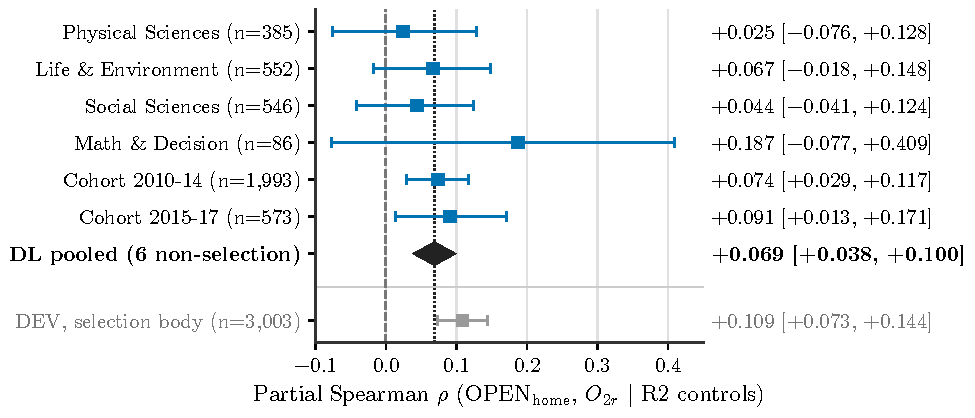
\includegraphics[width=\linewidth,height=0.85\textheight,keepaspectratio]{figures/fig_evidence_synthesis_v0.pdf}
  \caption{Partial Spearman correlation of OPEN$_{\text{home}}$ (home-neighbourhood openness over $t_0..t_0{+}2$) with rarefied cross-field breadth ($O_{2r}$, $m=50$) at ladder rung R2. R2 controls for the five-feature popularity baseline B5 plus onset year, contact reach, concept type, a generic-concept flag and concept level. Blue squares with whiskers show the estimate and 95\% concept-bootstrap CI (2{,}000 draws) for each of six non-selection bodies: four held-out home groups (Physical Sciences, Life \& Environment, Social Sciences, Math \& Decision; onsets 2003--09), the 2010--14 onset cohort and the 2015--17 onset cohort. $n$ is the number of concepts analysed. The black diamond spans the DerSimonian--Laird pooled estimate over these six bodies, $+0.069$ $[+0.038, +0.100]$, $I^2 = 0$, 6/6 positive. The dotted vertical line marks this pooled estimate and the dashed line marks zero. The grey row below the separator is the DEV selection body, on which the index was chosen ($+0.109$ $[+0.073, +0.144]$). It is not pooled, and it is $1.58\times$ the non-selection pool. Values at right are estimate [95\% CI]. The association is small and has the same sign in every body, but only the two cohort rows and the pool have CIs above zero individually. All non-selection bodies except the 2015--17 cohort had outcomes read in earlier analyses, so the pool is descriptive rather than confirmatory.}
  \label{fig:evidence_synthesis}
\end{figure}

\textbf{Vocabulary-free replication.} To address survivorship bias in the legacy concept vocabulary, we mined 636 vocabulary-free phrase-born concepts\footnote{Code: \url{https://github.com/ai-inventor-papers/ai-invention-8795ea-concepts-spread-once-adopters-make-them/tree/fork/run_-IpcIodNqp66/round-5/experiment-13}} (2003--2015 onsets). These newborns have 14\% lower breadth and 89\% higher transience than legacy concepts. On this vocabulary-free frame, OPEN$_{\text{home}}$ gives PSP +0.117 [+0.020, +0.218] at control rung R3 for $O_{2r}$ ($m = 30$); the verdict is partial: the most demanding rung's confidence interval includes zero (+0.086 [$-$0.009, +0.190]), three of four estimable groups are positive, and the Holm-corrected $p$-value is 0.052. The pre-declared secondary index NOVCHURN$_{\text{home}}$ is +0.108 [+0.007, +0.211] at R3 but its interval includes zero at R4 and R5. Edge persistence is null ($-$0.013); the signal is carried by neighbourhood novelty (NOV$_{\text{res}}$ +0.208 [+0.113, +0.303]). On this frame the coupling contrast is not significant (OPEN$_{\text{all}}$ minus OPEN$_{\text{home}}$ +0.056 [$-$0.024, +0.131]), and OPEN$_{\text{home}}$ adds no forecasting gain over B5.

\textbf{The consistency--breadth reversal.} We rebuilt \citeauthor{Cheng2023}'s (\citeyear{Cheng2023}) ideational consistency on OpenAlex topic co-usage for 12{,}311 concepts\footnote{Code: \url{https://github.com/ai-inventor-papers/ai-invention-8795ea-concepts-spread-once-adopters-make-them/tree/fork/run_-IpcIodNqp66/round-5/experiment-14}}. In their design (next-year volume, no current-size control), the model reproduces their estimate: $b = 0.428$ (+53.5\%/SD). Adding current volume removes almost all of it: +1.3\% [+0.5\%, +2.1\%], a residual-to-raw ratio of 0.021. Net of B5, the partial Spearman of consistency with rarefied breadth is $-$0.069 [$-$0.093, $-$0.047] on the pooled bodies ($I^2 = 0$, 5/5 groups negative), replicating on the 2015--2017 cohort ($-$0.111 [$-$0.197, $-$0.030]). The consistency measure has Spearman +0.77 with edge persistence (Jaccard similarity); it is essentially weighted persistence. A stable neighbourhood goes with growth mainly because it goes with current size, and net of size it goes with narrower breadth. These bodies are selection data; on the vocabulary-free frame the breadth association is $-0.064$ [$-0.159$, $+0.031$], so the reversal is not confirmed there. The size $\times$ consistency interaction on transience predicted by group-turnover arguments (stability helps small groups, turnover large ones) is null ($-0.001$ [$-0.021$, $+0.020$], $n = 11{,}473$), and consistency is unrelated to uptake and transience net of B5.

\subsubsection{Discussion of RQ1}

The confirmed indicators divide into two groups. Contact reach, retention ratio and the field-density measures capture a concept's position in the inter-field backbone and partly reflect a pre-onset footprint. Community count, neighbourhood novelty and ego density capture the topology of the early co-occurrence neighbourhood in the all-papers build, which includes off-home papers. The OPEN index combines these into a single measure of early openness. Part of their signal is early spread measured through the off-home papers: on the 2015--2017 cohort the home-only community count ($+0.002$ [$-0.071$, $+0.081$]) and participation ($+0.050$ [$-0.041$, $+0.133$]) are null, against $+0.161$ and $+0.145$ in the all-papers build, and the home-only signal comes from NOV$_{\text{res}}$ ($+0.134$) and low edge persistence ($-0.112$). On the vocabulary-free frame the home-only community count is also null ($+0.069$ [$-0.027$, $+0.166$]), but participation is positive ($+0.120$ [$+0.011$, $+0.223$]) and the all-minus-home contrast is not significant, so this coupling warning is not confirmed there. The practical forecasting gain is small: OPEN$_{\text{home}}$ adds only +0.002 Spearman on the fresh cohort. The indicators characterise structural preconditions for broad diffusion rather than providing individually actionable forecasts. In the home-only build the weakest held-out group is Physical Sciences (PSP +0.025; Life \& Environment +0.067, pooled +0.069); in the all-papers build Life \& Environment is the weakest held-out group (+0.071 vs +0.181 pooled), which a boundary analysis could not explain.


\subsection{By what routes do concepts spread across fields?}

\label{subsec:rq2_entry}
\subsubsection{Experimental setup}

We test whether relatedness to the fields currently retaining a concept predicts which field it enters next, using a conditional logit on concept-year risk sets with an independent frame of 11{,}841 concepts (6{,}978 entry events in 6{,}076 informative strata)\footnote{Code: \url{https://github.com/ai-inventor-papers/ai-invention-8795ea-concepts-spread-once-adopters-make-them/tree/fork/run_-IpcIodNqp66/round-3/experiment-7}}. The frame excludes all concepts used in the development-set frame construction. The specification was hash-sealed on the development set before held-out scoring. Pre-registered criteria include: pooled R3 CI above zero, positive in the majority of evaluable groups, volume-matched contrast CI above zero, retained-label permutation null rejected, backbone-rewiring null rejected, and dose-response non-negative.

\subsubsection{Comparison to related work}

\citet{Hidalgo2007} showed that product-space relatedness predicts economic diversification; the minimum conditional probability defines the standard proximity. \citet{Boschma2015} extended the principle of relatedness to regional and technological diversification, and \citet{Fitzgerald2021} showed how regional knowledge networks shape academic localisation. Our contribution is to test whether relatedness to the set of fields currently \emph{retaining} a concept predicts entry, beyond relatedness to the home field and conventional density measures. The key methodological distinction is that retention, not mere presence, defines the reference set.

\subsubsection{Results}

On the independent held-out frame, the retained-frontier coefficient is $d_0 = 0.322$ [0.291, 0.355] (1{,}000-draw concept bootstrap; R3 vs R2 likelihood-ratio 325.8, $p < 10^{-70}$; 3{,}162 held-out concepts). The result is positive in three of three evaluable held-out groups: Physical Sciences +0.148, Life \& Environment +0.401, Social Sciences +0.297. Mathematics \& Decision Sciences is null (+0.065 [$-$0.110, 0.234], 165 concepts). DerSimonian--Laird pooled $d_0$ = 0.243 [0.118, 0.368], $I^2 = 0.92$ (Table~\ref{tab:entry}, Figure~\ref{fig:entry}).

\begin{table}[!htbp]
\centering
\caption{Retained-frontier coefficient ($d_0$) from the conditional-logit model of field entry, by domain group and cohort. The pre-registered verdict is PARTIAL: criterion 5 (volume-matched CI $> 0$) fails.}
\label{tab:entry}
\small
\begin{tabular}{lccc}
\toprule
Model & $d_0$ & 95\% CI (concept bootstrap) & LR (R3 vs R2) \\
\midrule
Development set & 0.246 & [0.222, 0.271] & 365.6 \\
Held-out pooled & 0.322 & [0.291, 0.355] & 325.8 \\
Physical Sciences & 0.148 & [0.074, 0.219] & -- \\
Life \& Environment & 0.401 & [0.347, 0.458] & -- \\
Social Sciences & 0.297 & [0.245, 0.345] & -- \\
Math \& Decision Sci. & 0.065 & [$-$0.110, 0.234] & -- \\
2010--2014 cohort & 0.321 & [0.292, 0.347] & -- \\
\bottomrule
\end{tabular}
\end{table}

The retained-frontier coefficient survives the conventional RCA density ($D_{\text{rca}}$) and a share-weighted current presence density: adding $d_0$ after both rivals gives LR = 365.6 on DEV and 325.8 on held-out data, and on held-out data the $D_{\text{rca}}$ coefficient falls from 0.093 to 0.022 once $d_0$ enters. All three specificity tests reject their nulls after Holm correction (retained-label permutation $p = 0.001$; backbone-rewiring $p = 0.004$; node-label $p = 0.003$).

However, the pre-registered verdict is PARTIAL. The volume-matched contrast (comparing entry rates of retained versus entered-but-not-retained fields in the same volume cell) is null: $-$0.028 [$-$0.105, +0.046] on held-out data ($-$0.008 on DEV; Holm $p$ = 0.76). The dose response by retention age on held-out data is 0.098 / 0.075 / 0.304, which is not monotone. Under minimum-conditional-probability proximity \citep{Hidalgo2007} instead of PMI, the held-out $d_0 = -0.021$ ($p = 0.012$), while RCA density becomes strong (LR 246). Persistence is therefore confounded with volume, and the result is backbone-specific.

\textbf{Gateway centrality.} Gateway centrality does not predict field retention: on 8{,}515 held-out episodes, the increment is effectively zero ($\Delta$AUC $-$0.00001, 95\% CI [$-$0.0006, +0.0003]).

\textbf{Breadth decomposition.} On 3{,}188 DEV concepts\footnote{Code: \url{https://github.com/ai-inventor-papers/ai-invention-8795ea-concepts-spread-once-adopters-make-them/tree/fork/run_-IpcIodNqp66/round-4/experiment-12}}, the breadth gap between the top and bottom $O_{2r}$ terciles decomposes, in the unstratified variant, as: early contact diversity 77.9\%, frontier advance $-$4.6\% (broad concepts gain new fields at similar rates), and retention 26.8\%; exploration minus retention is 0.464 [0.407, 0.528]. The primary volume-stratified variant gives 76.0\% / $-$4.5\% / 28.5\% and a difference of 0.431 [0.371, 0.493]. Excluding Medicine (the pre-registered variant iv), the difference is 0.633 [0.537, 0.727] on DEV, 0.492 [0.403, 0.575] on the pooled held-out groups and 0.445 [0.358, 0.527] on the 2010--2014 cohort; DerSimonian--Laird over three held-out groups gives 0.504 [0.329, 0.679] ($I^2 = 0.76$). These shares are an accounting identity for the breadth outcome, not causal effects, because breadth and contact diversity share papers.

\textbf{Diffusion trajectories.} No discrete trajectory typology passes the naming rule. DTW $k$-medoids and HMM-based clustering on state sequences give an adjusted Rand index of 0.222. PCA reveals a continuum: PC1 (38.8\% of variance) is a breadth axis, PC2 (10.7\%) is a keep-versus-lose axis. Early openness correlates with PC1 beyond B5 (held-out partial 0.120 for the all-papers build and 0.060 for the home-only build, $I^2 = 0$) but not positively with PC2 (DEV partial $-$0.07 to $-$0.11).

\textbf{Sequence and closure tests.} A home-prominence half-peak vs off-home take-off test finds no signal beyond the mechanical lag (DEV excess $-$0.009 [$-$0.015, $-$0.003], held-out +0.011 [0.005, 0.016]). Intersection-born concepts take off later (HR 0.47 [0.42, 0.54]); their off-home take-off comes without a prior home-prominence peak on DEV and the 2010--2014 cohort (H-S1 pooled +0.076 [+0.024, +0.126]) but not on the older held-out groups (+0.001). A within-concept closure test\footnote{Code: \url{https://github.com/ai-inventor-papers/ai-invention-8795ea-concepts-spread-once-adopters-make-them/tree/fork/run_-IpcIodNqp66/round-5/experiment-15}} is null on the development set (density PPML $b = -0.070$ [$-$0.180, 0.040]; OPEN$_{\text{home}}$ $b = +0.015$ [$-$0.038, 0.069]). On held-out fields, OPEN$_{\text{home}}$ is opposite-signed ($-$0.079 [$-$0.146, $-$0.013]), and a Sun--Abraham event study around the first home closure jump is null (DEV lag 0--2: $-$0.018 [$-$0.042, +0.004]). Early openness is a between-concept trait, not a within-concept mechanism.

\begin{figure}[!htbp]
  \centering
  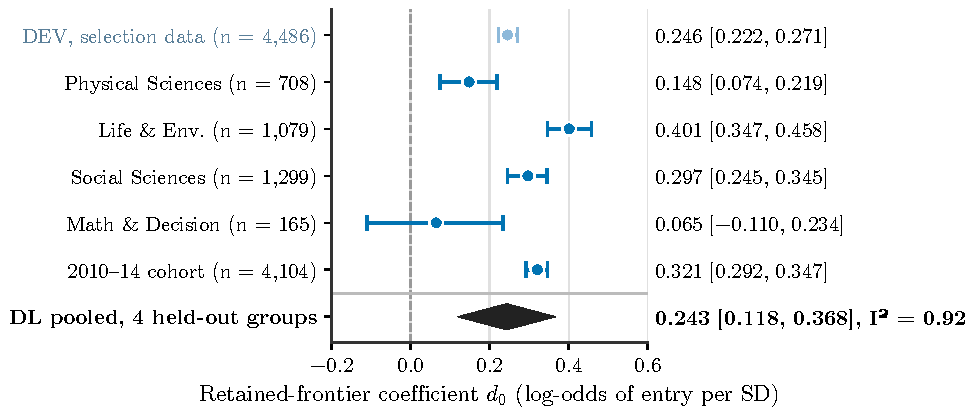
\includegraphics[width=\linewidth,height=0.85\textheight,keepaspectratio]{figures/fig_entry_v0.pdf}
  \caption{Retained-frontier coefficient $d_0$ (log-odds of entering a field per SD of relatedness to the off-home fields that currently retain the concept) from the conditional-logit entry model (rung R3, controlling for home relatedness, field size, entered density, own gateway centrality, RCA density $D_{\mathrm{rca}}$ and volume density $D_{\mathrm{vol}}$), by unit. Circles with bars show point estimates with 95\% concept-bootstrap confidence intervals. The light-blue row is the development (DEV) set used for selection. Dark-blue rows are the held-out domain groups and the 2010--14 onset cohort. The black diamond is the DerSimonian--Laird random-effects estimate pooled over the four held-out groups, and its width spans its 95\% CI. The right column prints each estimate and interval; $n$ is the number of concepts in each unit. The dashed line marks $d_0 = 0$. $d_0$ is positive with a CI excluding zero in all three evaluable held-out groups (Physical Sciences 0.148, Life \& Env.\ 0.401, Social Sciences 0.297) and in the cohort (0.321). Math \& Decision ($n = 165$, excluded as underpowered before the freeze) is null (0.065 [$-$0.110, 0.234]). The pooled estimate is 0.243 [0.118, 0.368] with high heterogeneity ($I^2 = 0.92$). The frozen verdict is nonetheless PARTIAL: the pre-registered volume-matched contrast is null, and the effect is specific to the PMI backbone.}
  \label{fig:entry}
\end{figure}

\subsubsection{Discussion of RQ2}

The retained-frontier result extends the principle of relatedness to concept adoption. The positive coefficient is large and consistent across three of three evaluable groups, but the PARTIAL verdict limits its interpretation: we cannot fully separate persistence from sustained volume as a predictor of field entry. The effect is also backbone-specific: it holds on the sparse PMI backbone but not under the standard Hidalgo proximity. The breadth decomposition shows that integrating and localised concepts differ primarily in how many fields they contact early, not in how many more fields they enter later. The null closure test and opposite-signed held-out result indicate that openness does not operate as a within-concept mechanism driving diffusion.


\subsection{Confound analysis}
\label{sec:confound}

The openness signal could be an artefact of small yearly samples or of dynamic churn. We tested four null models\footnote{Code: \url{https://github.com/ai-inventor-papers/ai-invention-8795ea-concepts-spread-once-adopters-make-them/tree/fork/run_-IpcIodNqp66/round-5/experiment-16}}:

\textbf{Fixed-size rarefaction.} Subsampling to 10 home papers per year retains 68\% of the pooled association. The bias-corrected Chao estimator retains 91\% (same-sample retention ratio 0.913).

\textbf{Within-concept permutation null.} The excess churn over a 200-draw within-concept year-label permutation null is indistinguishable from zero: excess NOVCHURN pooled PSP = +0.008 [$-$0.02, +0.03], compared to raw NOVCHURN = +0.116 [+0.09, +0.14]. The $R^2$ of raw persistence on the permutation-null mean is 0.66. What predicts breadth is a static property of the concept's home-topic partner mix.

\textbf{Degree-preserving configuration null.} Replacing raw ego density and persistence by configuration-null $z$-scores (backbone rewiring for density, curveball for persistence) raises OPEN$_{\text{home}}$ from +0.092 to +0.115.

\textbf{Reliability.} Split-half reliability of NOVCHURN$_{\text{raw}}$ is 0.48. The temporal-excess variants (V2) have split-half Spearman--Brown reliability of approximately 0.01--0.05, and the planted-churn check fails. The disattenuated pooled NOVCHURN PSP is 0.178 [0.141, 0.214] (approximate, CI not independently re-derived).

Because the V2 temporal-excess measure is unreliable, the analysis cannot adjudicate temporal churn at typical sample sizes ($\sim$10 home papers/year). The association that survives behaves like a static dispersion property. Temporal turnover is untested rather than refuted.

\textbf{Partner decomposition.} The home-only signal is carried by partners from new Leiden communities arriving through mixed-field papers: contrast $C_2$ = +0.102 [+0.069, +0.133] (Holm $p$ = 0.0025), domain Shapley $\phi$ = +0.132 on the 2015--2017 cohort (method = +0.012), although on the pooled selection frame method partners carry slightly more ($\phi$ +0.067 vs +0.051). The pre-registered H-P1 split holds for new- versus same-community partners (+0.216 [+0.081, +0.351]) but fails for method versus domain partners ($-$0.055 [$-$0.122, +0.011]). Controlling for the share of early bridging papers halves NOVCHURN from 0.118 to 0.056. These mechanism analyses use the legacy-vocabulary frames, not Frame~N.


\subsection{Exploratory AI-domain stage}

An exploratory retrospective atlas of 37 AI and computer science concepts was constructed from the large panel, describing the early ($t_0{-}3$ to $t_0{+}2$) co-occurrence neighbourhoods of concepts such as deep learning, convolutional neural networks, cloud computing and crowdsourcing, grouped by their later spread. This atlas is outcome-selected and retrospective; it provides qualitative context but no hypothesis-testing power.


\subsection{Representative case studies}

Seven matched case-study pairs were drawn from the breadth decomposition analysis (Table~\ref{tab:cases}; one pair is shown in Figure~\ref{fig:case_study}). Each pair takes a top-quintile and a bottom-quintile OPEN$_{\text{all}}$ concept from the same reporting group, matched on early volume, growth and onset year; in 7 of 7 pairs the high-OPEN member has the higher size-adjusted breadth. These pairs are illustration only; all are descriptive with no $p$-value.

\begin{table}[!htbp]
\centering
\caption{Representative matched case-study pairs, contrasting high-openness and low-openness concepts matched on early volume and growth. All pairs are illustration; no inferential claim is made.}
\label{tab:cases}
\small
\begin{tabular}{lll}
\toprule
High-OPEN concept & Low-OPEN concept & Group \\
\midrule
Graphics processing unit & Vertical-axis wind turbine & CS+Eng \\
Shotgun proteomics & Image-guided radiation therapy & BGM+Med \\
Nanocarriers & Nanosheet & PHYS \\
Soft power & Autonomous learning & SOC \\
Scopus & Oxygen reduction reaction & CS+Eng \\
Sclerostin & IgG4-related disease & BGM+Med \\
User-generated content & Mindfulness-based cognitive therapy & SOC \\
\bottomrule
\end{tabular}
\end{table}

\begin{figure}[!htbp]
  \centering
  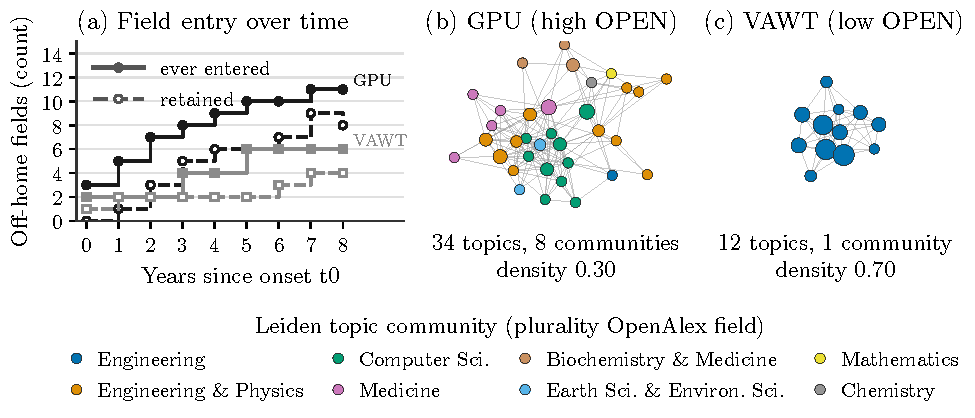
\includegraphics[width=\linewidth,height=0.85\textheight,keepaspectratio]{figures/fig_case_study_v0.pdf}
  \caption{Illustrative matched case-study pair (pair 1 of 7): graphics processing unit (GPU; onset $t_0=2008$, high early-neighbourhood openness OPEN) versus vertical-axis wind turbine (VAWT; $t_0=2009$, low OPEN). Both have an Engineering home field and are matched on early volume and growth. (a) Number of off-home venue fields each concept has ever entered (solid line, filled markers) and currently retains (dashed line, open markers) in each year from $t_0$ to $t_0+8$; GPU is shown in black and VAWT in grey on a shared axis. (b,~c) Topic co-occurrence ego networks over the first three years ($t_0$ to $t_0+2$, all papers). The nodes are the concept's positive-PMI neighbour topics (the concept itself is not drawn), the edges are links between those topics in the topic backbone, node area scales with the number of the concept's papers carrying the topic, and colour gives the topic's Leiden community, named by the plurality OpenAlex field. GPU's neighbourhood has 34 topics in 8 communities (density 0.30). VAWT's has 12 topics in a single Engineering community (density 0.70). The pair illustrates the openness--breadth association and is not evidence for it.}
  \label{fig:case_study}
\end{figure}


\subsection{Dead ends and negative results}
\label{sec:dead_ends}

Table~\ref{tab:deadends} lists the principal hypotheses and candidate signals that were tested and did not survive.

\begin{table}[!htbp]
\centering
\caption{Principal dead ends and negative results.}
\label{tab:deadends}
\small
\begin{tabular}{p{4.2cm}p{2.5cm}p{5.5cm}}
\toprule
Hypothesis / candidate & Decisive test & Result \\
\midrule
Naturalisation gap ($A^*_h$) & Indicator screen & Fails 3 of 4 pre-registered clauses ($\Delta\rho$ $-$0.006; only the size check passes) \\
$D_{\text{ratio}}$, $F_{\text{res}}$ & Ratio indicators & No candidate survives \\
Gateway centrality $\rightarrow$ field retention (H1) & Gateway analysis & $\Delta$AUC $-$0.00001 held-out \\
H3 gateway-weighted landing & Gateway analysis & Pooled CI includes 0 [$-$0.006, 0.065] \\
Ordering (central-first) & Trajectory analysis & MIXED: 32.6\% of broad concepts; negative lead-lag; pre-trend \\
Two discrete trajectory classes & Trajectory clustering & HMM-vs-DTW ARI 0.094/0.222 \\
Abandonment penalty ($d_{\text{lost}}$) & Entry model & Specification-dependent: A1 $-$0.007, R4 +0.064, min-cp $-$0.030 \\
Volume-matched retained-frontier contrast & Entry model & Null: $-$0.028 [$-$0.105, +0.046] held-out \\
$O_5$ external recognition & Indicator screen & No indicator beats B5 + onset year \\
Rescue and relay models & Trajectory analysis & Not supported \\
Within-concept closure & Closure test & Null on DEV; opposite-signed held-out ($-$0.079) \\
Early author count for $O_3$ & Cohort replication & Non-replication on fresh cohort (+0.014) \\
Retention ratio at R2/R3 & Cohort replication & Null on cohort ($-$0.043 [$-$0.116, 0.031]) \\
Trait prediction ($P$-B1) & Reliability test & Fails: yearly OPEN$_{\text{home}}$ ICC 0.34--0.39 \\
Vocab-free Cheng reversal & Vocab-free frame & Not confirmed ($-$0.064 [$-$0.159, 0.031]) \\
Co-author candidate S & Indicator screen & Computed; not confirmed for any outcome \\
\bottomrule
\end{tabular}
\end{table}


\section{Discussion}
\label{sec:discussion}

\subsection{What the openness index captures}

The OPEN index captures the degree to which a concept's early neighbourhood acquires partners from diverse communities rather than reinforcing existing ones. The signal is not demonstrably temporal turnover but a static topical-dispersion property. A within-concept permutation null absorbs the year-to-year component, yet the association persists: concepts whose home-field co-occurrence partners are novel, coming from communities that a degree-matched null does not expect, tend to reach more fields later (the home-only count of communities touched is itself null). This is consistent with \citeauthor{March1991}'s (\citeyear{March1991}) exploration--exploitation distinction at the concept level. However, the within-concept closure test is null on DEV and opposite-signed on held-out fields, indicating that openness operates as a between-concept trait rather than as a within-concept causal mechanism.

The home-only signal (OPEN$_{\text{home}}$) is marginal. The stronger OPEN$_{\text{all}}$ signal is partly mechanically coupled: early off-home papers that enter the ego network are a subset of the papers that determine the outcome. OPEN$_{\text{sizematch}}$ equalises paper counts but still includes off-home papers, so it does not remove the coupling; it lies between the two builds (OPEN$_{\text{sizematch}}$ minus OPEN$_{\text{home}}$ +0.053 [$-$0.015, +0.117]).

\subsection{Reconciling consistency and breadth}

\citet{Cheng2023} found that ideational consistency predicts a concept becoming ``core.'' We replicate their result for volume (+53\%/SD) but show that it is almost entirely a current-size effect (+1.3\%/SD once current volume is controlled) and that, net of the popularity baseline, the same property predicts \emph{narrower} cross-field reach. The reversal holds in all five field groups ($I^2 = 0$) and on the 2015--2017 cohort, all selection data, but it is not confirmed on the vocabulary-free frame ($-0.064$, CI includes zero). The features predictive of local consolidation and growth are distinct from, and partly opposed to, the features predictive of broad disciplinary spread.

\subsection{The retained-frontier claim}

The field-entry result ($d_0 = 0.322$ on the independent frame) extends the principle of relatedness from economic geography \citep{Hidalgo2007,Boschma2015} to concept adoption. The result is PARTIAL: the volume-matched contrast is null, and the effect is backbone-specific (it reverses under minimum-conditional-probability proximity). What survives is a PMI-backbone relative-odds effect that cannot be separated from volume. The $I^2$ of 0.92 indicates substantial cross-domain heterogeneity, with Life \& Environment showing the strongest signal and Mathematics \& Decision Sciences null.

\subsection{Limitations}

\textbf{Effect size.} The OPEN--breadth association is modest. OPEN$_{\text{home}}$ adds no forecasting gain over B5 (+0.002 [$-$0.003, +0.008]).

\textbf{Measurement noise.} Split-half reliability of OPEN$_{\text{home}}$ is 0.49. The temporal-excess variants have split-half reliability below 0.05, so temporal versus static dispersion cannot be resolved at available sample sizes.

\textbf{Vocabulary bias.} The legacy OpenAlex concept vocabulary is survivor-selected. Frame~N is small (636 concepts) with pre-unseal power of 0.47.

\textbf{Coupling.} About half of the OPEN$_{\text{all}}$ signal is mechanical coupling between the ego-network construction (which uses off-home papers) and the breadth outcome. OPEN$_{\text{home}}$ is free of this coupling but marginal.

\textbf{Domain heterogeneity.} The home-only OPEN signal is weakest in Physical Sciences (PSP +0.025); in the all-papers build Life \& Environment is weakest (+0.071). The retained-field relatedness $I^2$ is 0.92.

\textbf{Not causal.} Early ego-network openness could reflect a concept's intrinsic generality, the diversity of the research community around it, or the breadth of the problems it addresses.

\textbf{Prior unsealing.} Held-out outcomes were previously unsealed by two earlier experiments in the same project, so the indicator-screen held-out results are robustness checks.

\textbf{Scope.} The paper does not test the run's original lineage-assortativity (naturalisation-gap) measure beyond reporting it as a dead end, and it does not report the iteration-1 M1 background-homophily decomposition ($R^2$ 0.66) or the iteration-2 label-coverage artefact analysis; these are recorded in the internal report only. The planned Frame~N replications of the breadth decomposition, the PC1/PC2 split and the partner decomposition were not run.


\section{Conclusions}
\label{sec:conclusions}

We screened 53 early temporal network indicators for predicting the cross-disciplinary breadth of new scientific concepts, using 12{,}499 concepts from the OpenAlex corpus with held-out validation and a fresh-cohort test (marginal: R4/R5 and DerSimonian--Laird intervals include zero). Seven indicators are confirmed; from the ego-network family we build the OPEN index, which captures topical non-redundancy in a concept's early co-occurrence neighbourhood and has a small association with breadth (pooled +0.069) but no forecasting gain. The signal is a static between-concept trait; temporal turnover could not be tested at available sample sizes. Early openness is associated with breadth; early consolidation goes with volume even after controlling for current size (+0.094 [0.007, 0.186] on the vocabulary-free frame) and, net of volume, with narrower breadth on selection data (not confirmed on the vocabulary-free frame). Concepts spread next to fields related to those currently retaining them, but the pre-registered verdict is PARTIAL: persistence and volume are confounded, and the effect is backbone-specific.


\section*{Declarations}

\subsection*{Availability of data and materials}
\begin{sloppypar}
The study uses the publicly available OpenAlex bulk snapshot (2026-09-23). Analysis code is available at
\url{https://github.com/ai-inventor-papers/ai-invention-8795ea-concepts-spread-once-adopters-make-them/tree/fork/run_-IpcIodNqp66};
individual experiment folders are linked in the paper's footnotes. Concept frames and indicator matrices are available from the corresponding author upon request.
\end{sloppypar}

\subsection*{Competing interests}
The authors declare no competing interests.

\subsection*{Funding}
Not applicable.

\subsection*{Authors' contributions}
All authors contributed to the study design, analysis and manuscript preparation.

\subsection*{Acknowledgements}
Not applicable.

\bibliographystyle{plainnat}
\bibliography{references}

\end{document}
